\epigraph{An SQL query walks into a bar and sees two tables.\\
  He walks up to them and asks ``Can I join you?''}{\textit{– Source: Unknown,
    from~\cite{join_tjo}}}

In this chapter a background is given to relational databases, focusing on the
areas of interest for this thesis. The first section will give a high-level
introduction to relational databases and how they work in general. Following
this is a section with a more in-depth description of indexes. After this comes
the final section covering the query optimizer, detailing how it works, how it
can be monitored and its limitations.

\section{Relational databases}
A database is a computerized record-keeping system, a way to save computerized
data~\cite[p. 6]{date_2003_introduction_aitds}. The data stored in the database
can then be accessed and modified by the user. Accessing and modifying the data
is typically done through a layer of software called the database management
system, which provides a method for accessing and modifying the data.

A database stores data in the form of rows in different tables. These rows are
also sometimes referred to as tuples. In a relational database these tuples can
then have relations between each other in the form of for example ``Tuple A has
one or more of Tuple B''.

The following sections will describe some components of the database which are
of the most relevant for this thesis.  First comes a section describing the most
common language, SQL, when writing queries in relation languages, after this is
is a section describing how the query described by SQL is executed and finally a
section covering one of the most fundamental operations in SQL --- the join
operation.

\subsection{SQL}
SQL, or Structured Query Language in full, is the computer language most
commonly used to query and modify the database, it is formally defined by
ISO/IEC
9075~\cite[p.~29]{garcia-molina_2002_database_dstcb}\cite{iso_i9itdlsp1f}. The
language came from research into manipulating databases in the early '70s and it
is now one of the most popular database languages in existence~\cite{sql_s|cl}.

\subsection{Query execution}
The execution of a query in the form of an SQL-statement is split into four
phases~\cite{selinger_1979_access_apsiardms}:
\begin{enumerate}
\item \textit{Parsing}, in which the input text is transformed into query
  blocks;
\item \textit{Optimization}, in which an optimized way to access the data is
  found, called an \textit{access path};
\item \textit{Code generation}, in which the access path is transformed into a way to
  execute it, the \textit{execution plan};
\item And \textit{execution}, when the code is executed;
\end{enumerate}

The \textit{parsing}, \textit{code generation} and \textit{execution phases} are
all fairly trivial compared to the \textit{optimization}. The optimization
process is also the phase that has the potentially most effect on the execution
time for the query. The query optimization process is performed by the query
optimizer, which is described in more detail in Section~\ref{sec:queryopt}.

\subsection{The join operation}
One of the most fundamental operations in SQL is joining two tables. An
example of an inner join on the tables \sql{EMPLOYEES} and \sql{DEPARTMENTS} can
be found in Figure~\ref{fig:sql:joinop}.

\begin{figure}[ht]
  \begin{minted}[breaklines]{sql}
    SELECT *
    FROM   EMPLOYEES, DEPARTMENTS
    WHERE  EMPLOYEES.DEPARTMENT_ID = DEPARTMENTS.DEPARTMENT_ID
    AND    EMPLOYEES.NAME = 'John';
  \end{minted}
  \caption[An example of an SQL query]{An SQL query that will find the all
    employees by the name of John and info about their
    department.}\label{fig:sql:joinop}
\end{figure}

There are four kinds of joins typically supported in databases. To illustrate
this assume we have the following \texttt{Join(A, B)}, where \texttt{A} and
\texttt{B} are relations and \texttt{Join} is one of the join operations.
\begin{itemize}
\item An inner join will return all rows in common between \texttt{A} and
  \texttt{B};
\item A left outer join will return all rows in \texttt{A} and all common rows
  in \texttt{B};
\item A right outer join will return all rows in \texttt{B} and all common rows
  in \texttt{A};
\item And a full outer join will return all rows in \texttt{A} and all rows in
  \texttt{B}.
\end{itemize}
See Figure~\ref{fig:vennjoin} for a visualization of the joins using Venn
diagrams.

\begin{figure}[ht]
  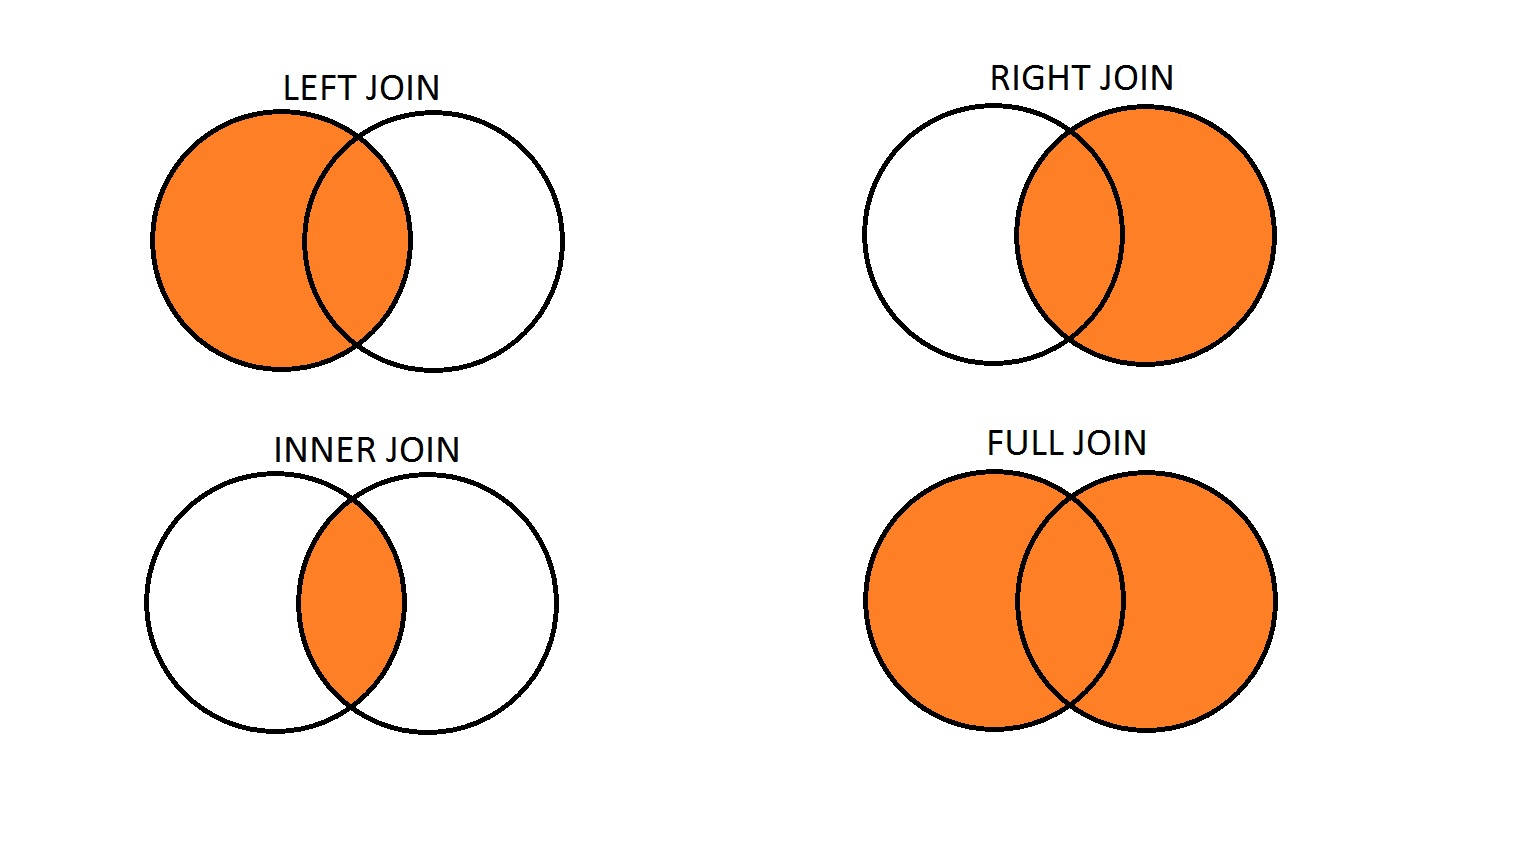
\includegraphics[scale=0.4]{Images/SQL-Join-Venn-Diagrams.jpg}
  \caption[Illustration of join operations using Venn diagrams]{The four join
    operations illustrated using Venn diagrams, image taken
    from~\cite{brian_2014_better_bqj}.}\label{fig:vennjoin}
\end{figure}

\subsection{Implementation of operators}\label{sec:opimpl}
Operators can be divided into three classes:
\begin{enumerate}
\item\label{item:classop:sort} \textit{Sorting-based} methods;
\item\label{item:classop:hash} \textit{Hash-based} methods;
\item\label{item:classop:index} And \textit{index-based} methods.
\end{enumerate}
In general index-based methods are variations of class~\ref{item:classop:sort}
or~\ref{item:classop:hash} that utilize indexes to speed up parts of the
algorithm. Most notably when there exists an index --- for example B-trees ---
that allows the data to be accessed sorted, joins can be done very efficiently.

Furthermore the algorithms for the operators can be grouped by the number of
passes the algorithm does:
\begin{enumerate}
\item \textit{One-pass algorithms} read the data from disk only once;
\item \textit{Two-pass algorithms} read the data once, process and then save
  it before doing another pass;
\item And algorithms that do three or more passes and are essentially
  generalizations of two-pass algorithms.
\end{enumerate}

There are several operators to implement in a database, but the most relevant
algorithms for this thesis are those implementing the join operator.
Implementation of the join operator is typically done with three fundamental
algorithms: nested loop join, merge join and hash join~\cite{postgresql_pd9p}.
Many databases support more join algorithms, but they are typically variations
of one of these three algorithms.

For the descriptions of the algorithms assume we have a query joining the tables
\texttt{A} and \texttt{B}, \texttt{Join(A, B)}. The first table of the join
operation, \texttt{A}, is referred to as the \textit{outer table} and the second
table, \texttt{B}, as the \textit{inner table}.

\subsubsection{Nested loop join}\label{sec:nestedloopjoin}
A nested loop join is essentially two nested loops, one over the outer table and
inside it one over the inner
table~\cite[p.~718-722]{garcia-molina_2002_database_dstcb}. The nested loop join
is a bit of a special case as it is not necessarily of any of the classes. The
number of passes it does can also be considered to be ``one-and-a-half'' as the
outer table's tuples is read only once, while the inner table's tuples are read
repeatedly.

If an index exists for the inner table the nested loop join could be considered
to be of class~\ref{item:classop:index} and is then called a \textit{index
  nested loop join}.

\subsubsection{Merge join}
A merge join (sometimes also called \textit{sort-merge join}) is a variation of
a nested loop join that requires both tables to be sorted. The two tables can
then be scanned in parallel, allowing each row to only be scanned
once~\cite[p.~723-730]{garcia-molina_2002_database_dstcb}. The sorting of the
tables can be achieved through an explicit sort step or through an index.

A merge join can be considered to be a two-pass algorithm of
class~\ref{item:classop:sort}.

\subsubsection{Hash join}
There are several types of hash joins but the general principle remains the
same: build a hash table for the outer table, then scan the inner table to find
rows that match the join
condition~\cite[p.~732-738]{garcia-molina_2002_database_dstcb}.

Hash joins are two-pass algorithms of class~\ref{item:classop:hash}.

\section{Indexes}
This section will cover the basics behind indexes as described by Ramakrishnan
et.\ al.\ in~\cite[Ch.~8]{ramakrishnan_2003_database_dms}.

An index is a data structure that allows data stored in the database to be
accessed more efficiently for some retrieval operations. The data stored in the
index is called the \textit{data entry} and the value that is indexed --- the
value in the column --- is called the \textit{search key}. There are three
alternatives for what to store as the data in the data entry:

\begin{enumerate}
\item\label{item:indexes:alt1} A data entry is a the actual data saved;
\item\label{item:indexes:alt2} A data entry is a pair containing a search key
  and record id;
\item\label{item:indexes:alt3} A data entry is a pair containing a search key
  and a list of record ids corresponding to the key.
\end{enumerate}

Which alternative is used depends on how the index is created and what kind of
an index it is.

\subsection{Compound indexes}
Compound indexes are indexes containing more than one fields. A compound index
can support a broader range of queries than a normal index and since they also
contain more columns, they contain more information about the data saved.

\subsection{Clustered index}
A clustered index is an index on a column which is sorted in the same way as the
index; otherwise it is an unclustered index. An index using
Alternative~\ref{item:indexes:alt1} is sorted by definition, whereas
Alternative~\ref{item:indexes:alt2} and~\ref{item:indexes:alt3} require the data
stored to be sorted.

\subsection{Data structures}
The two most common indexes used are \textit{hash-based indexes} and
\textit{tree-based indexes}. Below is a more detailed description of both.

\subsubsection{Hash-based indexes}
A hash-based index is implemented as a hash table, mapping the hashed value of a
search key to a bucket containing one or more values. To search in the index the
search key is hashed and the corresponding bucket is identified, all values in
the bucket are then examined to identify the matching one.

\subsubsection{Tree-based indexes}
Tree-based indexes save the data as hierarchical sorted trees where the leaf
nodes contain the values. To find a value the search starts at the root and all
non-leaf nodes direct the search toward the correct leaf node. In practice the
trees are often implemented as $B^{+}$-trees, which is a data structure that
ensure that paths from the root to a leaf node are of the same
length~\cite{comer_1979_ubiquitous_ub}. The efficiency of a B-tree index depends
on the number of levels the B-tree
has~\cite[p.~645]{garcia-molina_2002_database_dstcb}.

\section{The query optimizer}\label{sec:queryopt}
In order to access the data in an efficient way, the query is optimized by a
built-in tool in the database called the query optimizer. Below is a
description of the fundamental operations performed by query optimizer, taken
mostly from C., Surajits article on the
topic~\cite{chaudhuri_1998_overview_aooqoirs}.

Query evaluation is handled by two components: the \textit{query optimizer} and
the \textit{query execution engine}. The input to the query optimizer is a
parsed representation of the SQL~query and the output is an access path, that is
transformed into a query plan that the query execution engine then performs.

In order for the query optimizer to find an access path it must be able to:
\begin{enumerate}
\item Expand the \textit{search space} to find all access paths that are valid
  transformations of the query;
\item Perform a \textit{cost estimation} for each access path to calculate its
  cost;
\item And finally \textit{enumerate} the access paths to find which is the best.
\end{enumerate}

A good query optimizer is one that does not cause too much overhead in the query
execution in calculating the access path, while still finding a good access
path. In order to do this each step must fulfill the criteria:
\begin{enumerate}
\item The search space includes plans with a low cost;
\item The cost estimation is accurate;
\item And the enumeration algorithm is efficient.
\end{enumerate}

\subsection{Expanding the search space}
The first task of the query optimizer is that of taking the original search
space containing just the original query, and expanding it through
transformation rules. The expansion will thus generate a larger search space
containing valid permutations of the join order. The output is a set of
\textit{operator trees}, which are binary trees where nodes represent operations
and leaves values.

There are multiple rules that can be applied, most of which are complex and work
only under some specific conditions. The most relevant rules for index-selection
are described below, for a more in-depth description
see~\cite{chaudhuri_1998_overview_aooqoirs}.

\subsubsection{Join reordering}
One important rule is that both inner join and full join are:
\begin{itemize}
\item \textit{Commutative}, \texttt{Join(R1, R2)} is equivalent to \texttt{Join(R2, R1)};
\item And \textit{associative}, \texttt{Join(R1, Join(R2, R3))} is equivalent to
  \texttt{Join(Join(R1, R2), R3)}.
\end{itemize}
This means that the joins can be grouped and reordered as the optimizer finds
best. Another consequence of this is that the operators that can be seen as a
single node with many children, see Figure~\ref{fig:groupop} for an example.

\begin{figure}[ht]
  \begin{subfigure}[b]{0.4\linewidth}
    \centering
    \begin{forest}
      [\texttt{JOIN}
      [\texttt{JOIN}
      [\texttt{JOIN}
      [\texttt{R}]
      [\texttt{JOIN}
      [\texttt{S}]
      [\texttt{T}]]]
      [\texttt{U}]]
      [\texttt{JOIN}
      [\texttt{V}]
      [\texttt{W}]]]
    \end{forest}
    \caption{\label{fig:groupop:a}}
  \end{subfigure}
  \begin{subfigure}[b]{0.4\linewidth}
    \centering
    \begin{forest}
      [\texttt{JOIN}
      [\texttt{JOIN}
      [\texttt{R}]
      [\texttt{S}]
      [\texttt{T}]]
      [\texttt{U}]
      [\texttt{V}]
      [\texttt{W}]]
    \end{forest}
    \caption{\label{fig:groupop:b}}
  \end{subfigure}
  \caption[An example of how operators can be grouped into a single node]{The
    \texttt{JOIN} operator is associative and commutative, allowing the access
    path in Figure~\ref{fig:groupop:a} to be transformed into
    Figure~\ref{fig:groupop:b}, example taken
    from~\cite[p.~791]{garcia-molina_2002_database_dstcb}.}\label{fig:groupop}
\end{figure}

\subsubsection{Pushing operations up and down the tree}
Another fundamental rule used by optimizers is that of pushing an operator down
the expression tree in order to reduce the cost of performing
it~\cite[p.~768-792]{garcia-molina_2002_database_dstcb}. For the example the
selection operators tend to reduce the size of the relations, meaning pushing
them down as far down the tree as possible is beneficial.

Another rule that can be applied is to pull an operator up the tree, in order to
then be able to push it down again to reduce the size of more relations. See
Figure~\ref{fig:pushop}, which illustrate how pulling a selection up the tree
allows it to then be pushed down more branches.

The conditions for when these rules are applicable naturally varies a lot
depending on the operator and it is beyond the scope of this thesis to list them
all. See~\cite[p.~768-779]{garcia-molina_2002_database_dstcb} for an in-depth
description of the rules and conditions.

\begin{figure}[ht]
  \begin{subfigure}[b]{0.4\linewidth}
    \centering
    \begin{forest}
      [\texttt{starName, studioName}
      [\texttt{JOIN}
      [\texttt{year = 1996}
      [\texttt{Movies}]]
      [\texttt{StarsIn}]]]
    \end{forest}
    \caption{\label{fig:pushop:a}}
  \end{subfigure}
  \begin{subfigure}[b]{0.4\linewidth}
    \centering
    \begin{forest}
      [\texttt{starName, studioName}
      [\texttt{JOIN}
      [\texttt{year = 1996}
      [\texttt{Movies}]]
      [\texttt{year = 1996}
      [\texttt{StarsIn}]]]]
    \end{forest}
    \caption{\label{fig:pushop:b}}
  \end{subfigure}
  \caption[Illustrating how operators can be pushed and pulled up and down the
  tree]{An expression tree representing a query to find which stars worked for
    which studios in 1996, example taken
    from~\cite[p.~774]{garcia-molina_2002_database_dstcb}. The selection
    operator in Figure~\ref{fig:pushop:a} is first pulled up the tree, allowing
    it to then be pushed down an additional branch as illustrated in
    Figure~\ref{fig:pushop:b}.}\label{fig:pushop}
\end{figure}

\subsubsection{Eliminating operators via an index}
Several operations such as \sql{GROUP BY}, \sql{ORDER BY}, \sql{MAX} etc can be
eliminated because the the relation is known to already fulfill these
criteria~\cite[p.~777-779]{garcia-molina_2002_database_dstcb}. One of the more
common criteria is the existence of an index that allows the data to be
retrieved sorted.


In combination with the ability to move operators up and down the tree this can
be very powerful as potentially costly operations can be eliminated.

\subsubsection{Accessing table data}
For each read from a table there will be generated one access path per usable
index, as well as one for a full table
scan~\cite[p.~827-829]{garcia-molina_2002_database_dstcb}.

\subsection{Cost estimation}
The second task of the query optimizer is to be able to assign a cost to a given
search plan. This cost estimation will be repeated several times for each
operator tree in the search space that the query optimizer considers relevant,
thus it is important that the estimation is efficient. The cost estimation is
done in three steps:
\begin{enumerate}
\item Collect statistics of stored data;
\item For each node in the tree, calculate the cost of applying the operation;
\item And then the calculate the statistics for the resulting output.
\end{enumerate}

Steps 2 and 3 are described in more detail
in~\cite{chaudhuri_1998_overview_aooqoirs} and are less relevant for this
thesis. Instead, the following section will focus on the first step ---
collecting statistics of the stored data.

\subsubsection{Collecting statistics}\label{sec:collecting_statistics}
There are two important statistics that need to be calculated for the data: the
number of tuples in a relation and the cardinality for each column in a relation
~\cite[p.~807-808]{garcia-molina_2002_database_dstcb}. However, the exact
cardinality is often impossible to calculate in a modern database as they often
contain huge amounts of data, making it practically impossible to calculate the
exact value.

Instead, the cardinality is estimated through
sampling~\cite[p.~807-808]{garcia-molina_2002_database_dstcb}. The idea is to
sample a fraction of the data and from that data generate an approximation of
the cardinality.

Approximating the cardinality is however not trivial --- it leads to the question
of what assumptions are done regarding the data, is it for example assumed to be
distributed uniformly? As described in
Section~\ref{sec:improving_cardinality_estimates}, modern databases often make a
simple assumption of independence --- an assumption which is often incorrect.

Regardless of the complexities of approximating, the intuitive idea is that if
we when sampling observe only a few different values for a relation, it
seems likely that we have seen most of the values for that relation --- indicating
a low cardinality. If we on the other hand observe almost only different
values, it is likely that it is instead the case that the relation has a high
cardinality.

\subsection{Enumeration}
The enumeration is the final task of the optimizer and the one that will perform
the actual expansion and cost estimation, as it selects in what way to expand
the search space. It would be too costly to expand the entire search space and
for each plan estimate the cost, instead the search space is expanded
heuristically in a way that the optimizer believes will identify the fast access
paths.

When expanding the search space the general principle is to find paths where the
size of relations is reduced as early as possible. For example pushing an
operation down the tree, as shown in Figure~\ref{fig:pushop}, can reduce the
size of the relation and thus reduce the cost of performing a join later
on~\cite[p.~772-774]{garcia-molina_2002_database_dstcb}.

If the enumeration algorithm estimates the cost for a new plan to be more
expensive than a previously found one, it can discard it right away. The main
goal for the enumeration algorithm is therefore to expand the search space in
such a way that the best plans are generated early, so that the more expensive
plans can be discarded quickly later on~\cite{nica_2012_analyzing_aqoppojea}.

Most modern query optimizers use a dynamic programming algorithm first proposed
in 1979 for the System R database~\cite{selinger_1979_access_apsiardms}. The
algorithm is built on the observation that the joins are independent ---
the $i$th join is independent of how the first $i-1$ relations were
joined. Based on this it is possible to construct a tree of all permutations of
joins by searching from smaller to successively larger subsets.

One final optimization done during this step is to heuristically prune
subtrees that the are deemed too bad to even
consider~\cite{ono_1990_measuring_mtcojeiqo}.

\subsection{Monitoring}
It is often useful to monitor and see what decisions the query optimizer make
and why; most databases implement the ability to do so via an
SQL-statement~\cite[p. 34]{lahdenmaki_2005_relational_rdidatodossea}. In
PostgreSQL and MariaDB the statement is called
\sql{EXPLAIN}~\cite{postgresql_pd9e}~\cite{explain_emkb}, but it is also called
\sql{SHOW PLAN} or \sql{EXPLAIN PLAN}. For an example of how \sql{EXPLAIN} is
used see Figure~\ref{fig:sql:explainquery}, which shows the code for a query,
and Figure~\ref{fig:sql:explaintrace}, which shows the corresponding trace.

\begin{figure}[ht]
  \begin{minted}[breaklines]{sql}
    EXPLAIN
    SELECT  title.title
    FROM    movie_info, title
    WHERE   movie_info.info IN ('Bulgaria') AND movie_info.movie_id=title.id;
  \end{minted}
  \caption[An example query to \sql{EXPLAIN}]{An example of a query done on the
    IMDb dataset, requesting the title of all movies filmed in Bulgaria. See
    Figure~\ref{fig:sql:explaintrace} for the
    output.}\label{fig:sql:explainquery}
\end{figure}

\begin{figure}[ht]
  \begin{lstlisting}
    Merge Join  (cost=2.25..921735.28 rows=19682252 width=17)
    Merge Cond: (title.id = movie_info.movie_id)
    ->  Index Scan using title_pkey on title  (cost=0.43..155884.96 rows=3572150
    width=21)
    ->  Index Only Scan using movie_info_idx_mid on movie_info
    (cost=0.44..511110.22 rows=19682252 width=4)
    (4 rows)
  \end{lstlisting}
  \caption[An example of an \sql{EXPLAIN} trace]{The access path as shown by
    PostgreSQL's EXPLAIN statement, corresponding to the the query in
    Figure~\ref{fig:sql:explainquery}. The output shows for example that the
    relation \texttt{title} is read with an \texttt{Index Scan} using
    \texttt{title\_pkey}, which is an index.}\label{fig:sql:explaintrace}
\end{figure}

\subsection{Limitations}
Even though much work has been done on improving query optimizers they may not
always choose the best access path. This section will describe some of the
primary reasons why an incorrect access path path is chosen, as described
in~\cite[Ch.~14]{lahdenmaki_2005_relational_rdidatodossea}.

\subsubsection{The optimizer can't see the best path}
One reason the query optimizer cannot find the best path is because it is unable
to see all alternatives because the query is too complicated.

\begin{itemize}
\item If a predicate is non-indexable it cannot by definition participate in
  defining the index slice. Furthermore it might also be the case when the
  predicate is even more difficult that the the optimizer is unable to perform
  an index screening, forcing it to read a table row.
\item If a compound predicate contains \sql{OR} it may become non-BT, which in
  turn means the predicate cannot be used to define the index slice. This means
  the query optimizer cannot make full use of potential indexes that exist.
\item Sometimes the optimizer will add an \sql{ORDER BY} to data that is already
  sorted thanks to an index.
\end{itemize}

\subsubsection{The optimizer's cost estimate is wrong}
Even if the optimizer is able to see all alternatives it might be the case that
the filter factor is incorrectly estimated, resulting in an incorrect access
path.

\begin{itemize}
\item If the filter factor is not estimated for a host variable, it must use a
  default value which often results in a poor estimate. However, if the filter
  factor is estimated every time the query is executed it adds a large
  overhead.
\item If the optimizer is unaware of the true distribution of the data it is
  forced to guess cardinality, a guess that tends to be wrong if the
  distribution of the data is skewed;
\item In a compound predicate such as \sql{HEIGHT = :HEIGHT AND WEIGHT =
    :WEIGHT} the optimizer can only produce a good estimate of the filter factor
  if it knows the cardinality of the combination of the \sql{HEIGHT} and
  \sql{WEIGHT} columns. If it does not, it must estimate this.
\end{itemize}
